% One Call is All You Need: Efficient KGQA via Question-Type-Guided Path Ranking
\documentclass[conference]{IEEEtran}

\usepackage{cite}
\usepackage{amsmath,amssymb}
\usepackage{graphicx}
\usepackage{booktabs}
\usepackage{multirow}
\usepackage{tabularx}
\usepackage{xcolor}
\usepackage{algorithm}
\usepackage{algorithmic}
\usepackage{enumitem}
\usepackage{hyperref}
\usepackage{subcaption}
\usepackage{adjustbox}
\usepackage{pifont}

\newcommand{\cmark}{\ding{51}}
\newcommand{\xmark}{\ding{55}}
\newcommand{\model}{\textsc{APR}}

\title{One LLM Call Is Enough: Adaptive Path Ranking for Efficient KGQA}

\author{\IEEEauthorblockN{Anonymous Authors}}
\begin{document}
\maketitle

\begin{center}
    \textbf{Abstract}
\end{center}
Knowledge Graph Question Answering (KGQA) aims to answer natural language questions by reasoning over structured knowledge graphs (KGs). Large Language Models (LLMs) have significantly advanced this field by acting as autonomous agents that iteratively plan and reason to navigate the graph. Current state-of-the-art methods typically employ such agentic workflows, requiring 5--10 LLM calls per query to perform planning, retrieval, and reflection. However, this multi-call paradigm suffers from high latency and computational cost, which derives in the retrieved graph structures can often be overly complex or lack the fine-grained detail necessary for precise reasoning. To address these issues, we propose \model{}, a novel framework that distills the complex reasoning process into a single-pass dense retrieval model.
Specifically, we employ a question-type classifier to predict reasoning complexity and guide candidate generation over adaptive subgraphs, followed by a late-interaction ranker with hop-aware position embeddings to identify the correct reasoning path in a single step. Experiments on WebQSP and ComplexWeb Questions demonstrate that \model{} achieves competitive accuracy compared to agentic methods while reducing LLM calls to exactly one and decreasing latency by \textbf{2--8$\times$}.
%Knowledge Graph Question Answering (KGQA) requires both semantic understanding of natural language and structured reasoning over large-scale knowledge graphs. Current state-of-the-art solutions adopt agentic Large Language Model (LLM) architectures that iteratively plan reasoning steps, retrieve subgraphs, and reflect on intermediate results through 5–10 LLM calls per query. However, this multi-call paradigm incurs prohibitive latency (1–2 seconds), suffers from cascading errors across iterations, and faces escalating API costs that fundamentally preclude real-time deployment.

\begin{IEEEkeywords}
Knowledge Graph Question Answering, Efficient Inference, Path Ranking, Question Classification
\end{IEEEkeywords}

%==============================================================================
\section{Introduction}
\begin{figure}[!t]
\centering
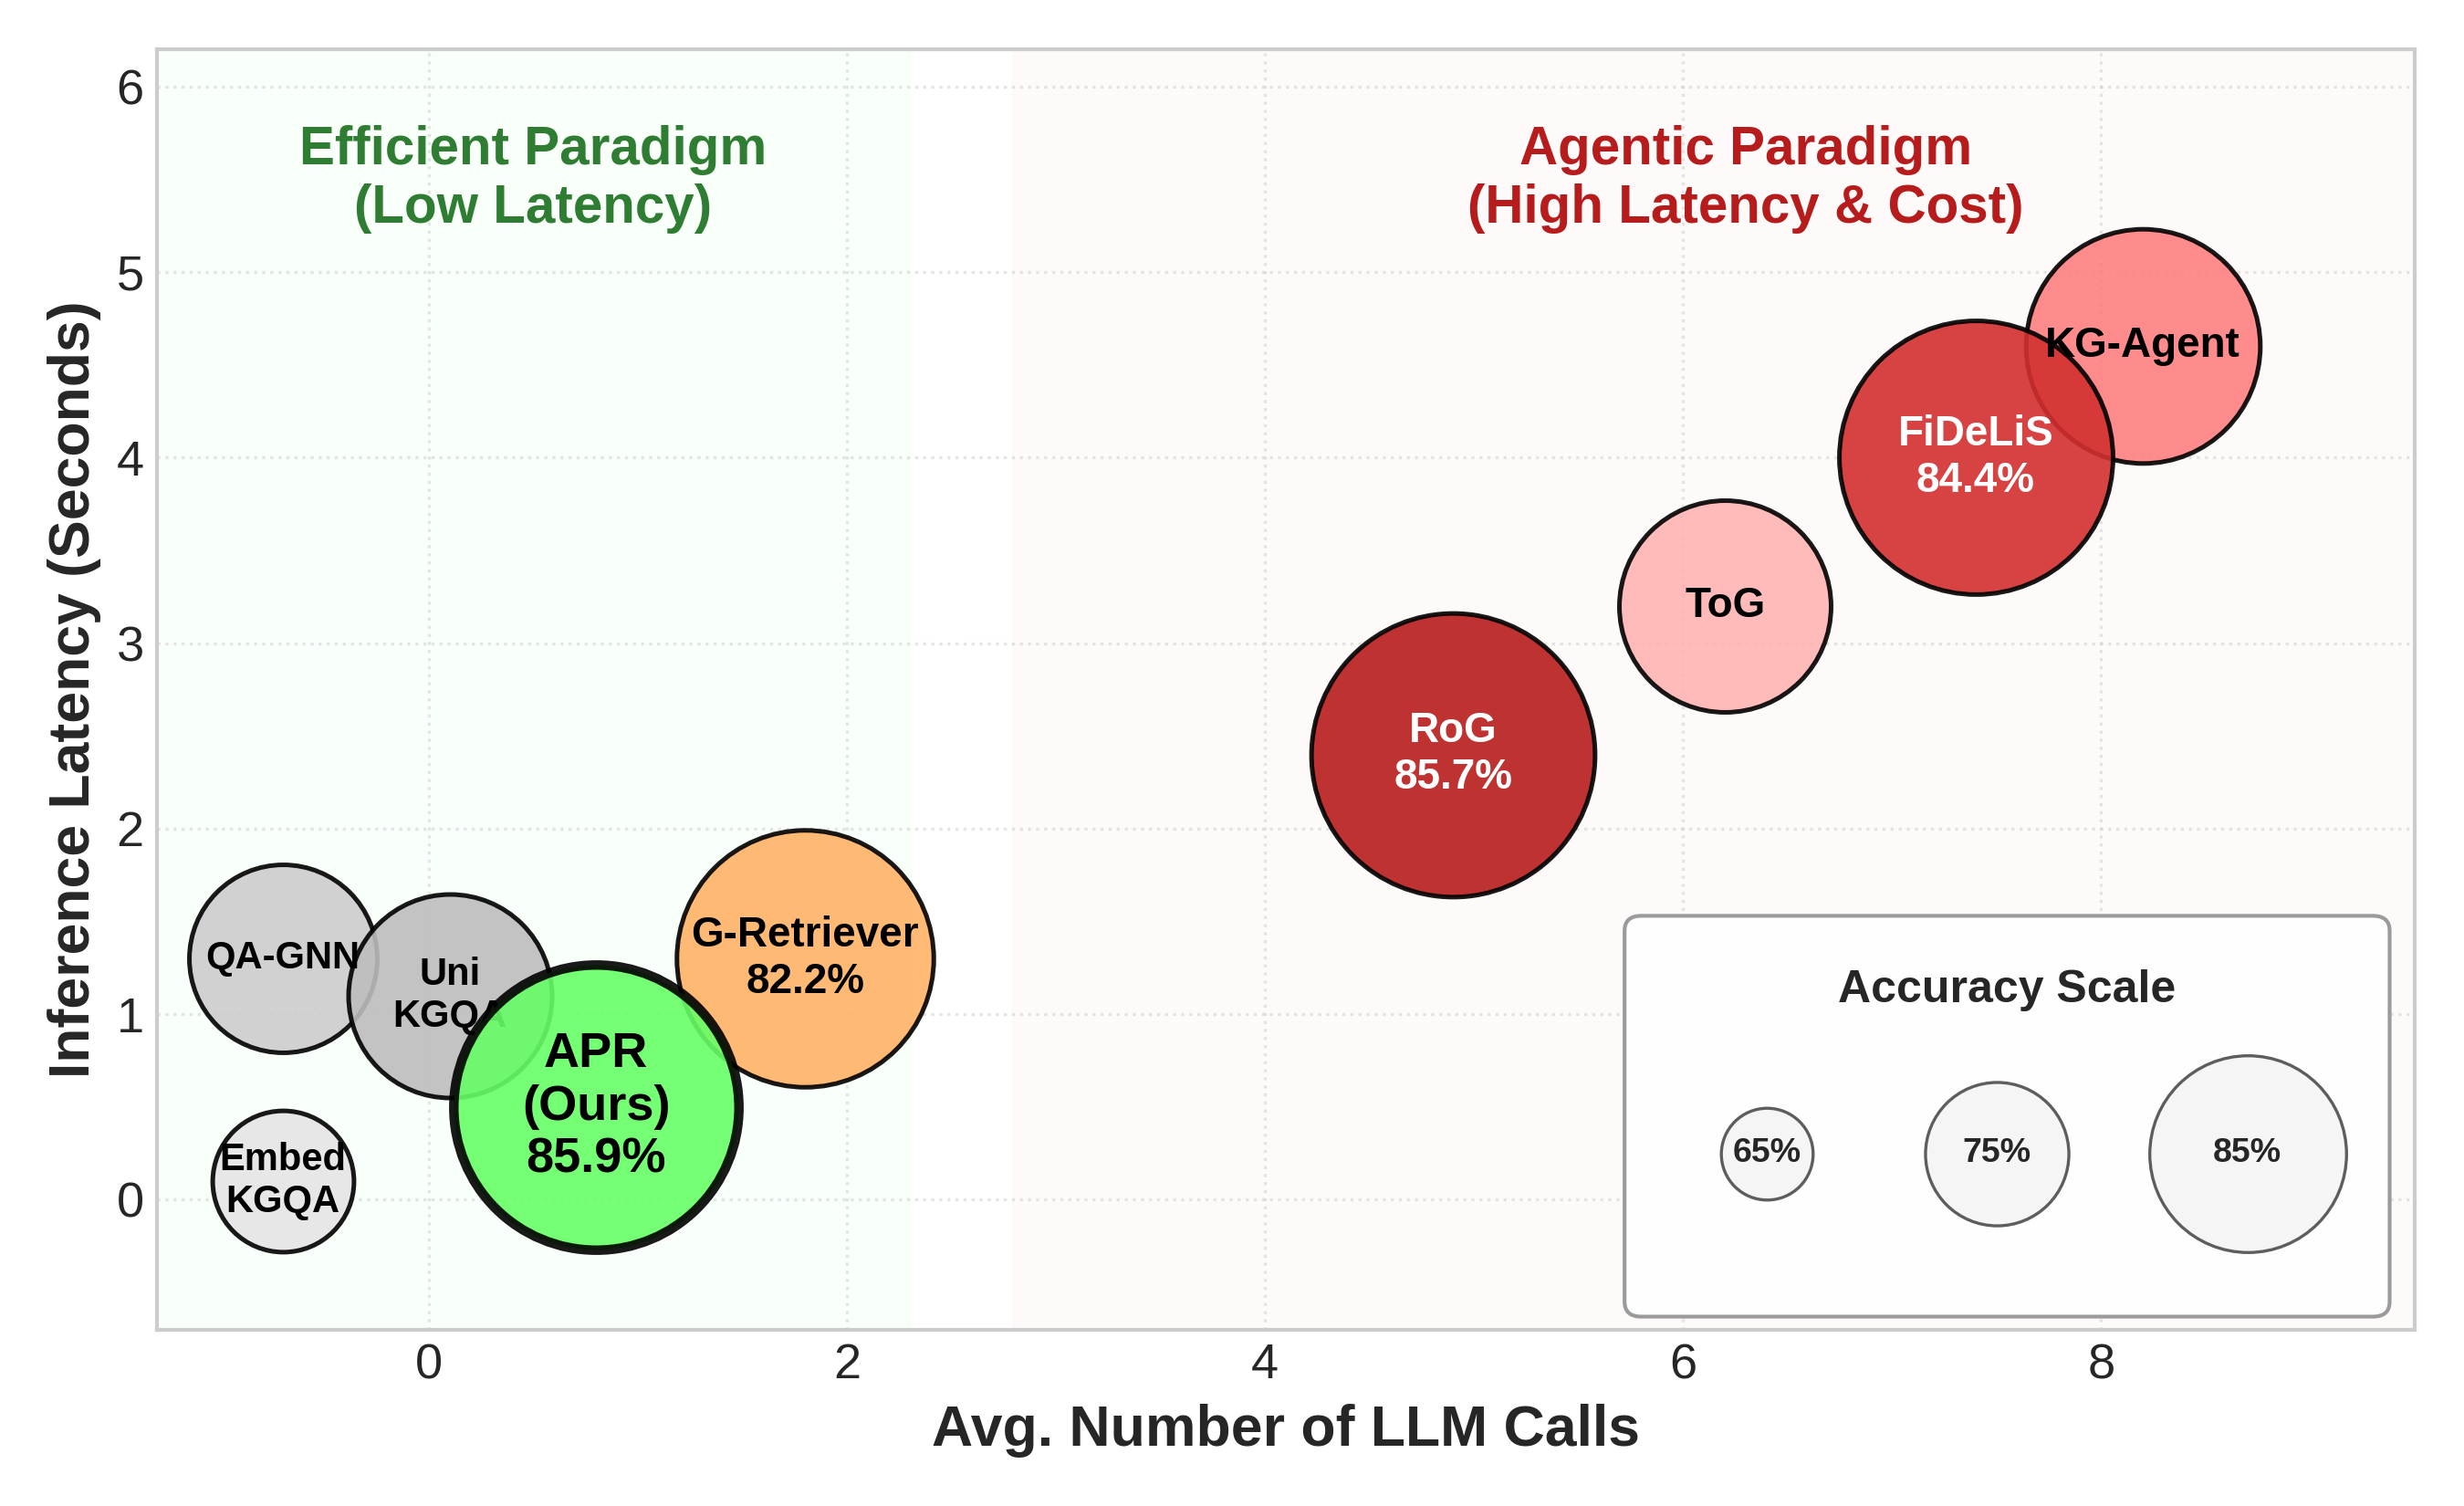
\includegraphics[width=\columnwidth,keepaspectratio,scale=1.2]{figures/figure1_tradeoff.png}
\caption{Comparison of KGQA Paradigms. The x-axis represents the number of LLM calls, the y-axis represents latency (lower is better), and the bubble size represents accuracy. \model{} (Ours) occupies the ideal “sweet spot”: high accuracy with minimal calls and low latency, contrasting with agentic methods (high cost/latency) and traditional embedding methods (lower accuracy).}
\label{fig:paradigm_bubble}
\end{figure}
%==============================================================================

Knowledge Graph Question Answering (KGQA) serves as a critical interface between human users and vast structured knowledge bases, requiring KGQA systems to understand natural language queries and perform multi-hop reasoning over graph structures \cite{ji2022kgsurvey, lan2021kbqasurvey, chakraborty2021intro}. The integration of Large Language Models (LLMs) has significantly advanced the field, enabling KGDA systems to handle increasingly complex questions with greater semantic understanding \cite{pan2024kg-llm-survey}.

Current state-of-the-art approaches predominantly follow an agentic paradigm \cite{sun2024tog, jiang2024kgagent, luo2024rog}. These methods typically operate through a sequence of steps where the LLM first decomposes the question via iterative planning and then dynamically retrieves subgraphs \cite{he2024gretriever}. While impressive, this paradigm relies on multiple sequential LLM calls (often 5--10 per query), leading to prohibitively high latency and computational costs \cite{sui2025fidelis}. Furthermore, dynamically retrieved subgraphs often contain irrelevant information, obscuring the correct reasoning path \cite{mavromatis2024gnnrag}. The ambition to achieve "one-call" KGQA is driven by the need for real-time responsiveness. Previous methods fail to achieve this: embedding-based methods \cite{saxena2020embedkgqa, jiang2023unikgqa} often lack the semantic depth to handle complex queries, while GNN-based approaches \cite{yasunaga2021qagnn} require expensive message passing. 
%如图1所示，一般会说大多数的方法，在需要好的性能的同时，存在需要多个CALL的，需要在一个复杂的图里面多次推理。于xxx,需要one call 同时保证性能， % 因为需要在一个复杂的图里面多次推理。 图过于简单，容易丢失细节。

%在这里我一般会说大多数的方法，在需要好的性能的同时，为了解决呢个问题，存在需要多个CALL的，如图1所示，，因此迫切的需要提出一种方法，去保留性能的同时减少CALL，agent 必须需要很多call 嘛？ 是不是因为需要在一个复杂的图里面多次推理。
%由于xxx,需要one call 同时保证性能， % 图过于简单，容易丢失细节。
%在这里我会加一个动机，也就是为什么这么做，比如究其本质，其需要多步的原因是因为graph不够细致，不符合问题，因此，我们由此提出了一个方法，xxx. 从而实现xxx.图1 所示。

% 受此启发，
Our goal is to shift the reasoning burden from the LLM to a specialized, structurally-aware retriever that can identify the gold path in a single forward pass, similar to dense retrieval advances in open-domain QA \cite{karpukhin2020dpr, khattab2020colbert}. Figure \ref{fig:paradigm_bubble} illustrates this landscape, highlighting how \model{} occupies a unique “sweet spot” by combining the high accuracy of agentic systems with the low latency of shallow retrievers.%

% 下面这段话好像是不必要的 ，或者是重复的， 应该就是一段话介绍我们具体咋做的，
Moreover, the environmental impact of complex AI systems is a growing concern \cite{schwartz2020green, strubell2019energy}. Agentic workflows that trigger 5--10 LLM calls per query linearly multiply energy consumption. By reducing the inference process to a single LLM invocation, \model{} directly aligns with the sustainable principles of Green AI.
%然后怎么做了实验，结果如何。
As shown in Figure~\ref{fig:architecture}, we propose \model{}, a streamlined framework that eliminates iterative LLM calls during reasoning. \model{} utilizes a question-type classifier to guide a targeted candidate generation process, followed by a late-interaction ranker augmented with hop-aware position embeddings. Our work makes three main contributions. First, we introduce a question-type guided candidate generation strategy that drastically reduces the search space by predicting reasoning complexity before path enumeration. Second, we develop a hop-aware late interaction ranker that captures structural alignment between questions and relation paths without requiring iterative generation. Third, we demonstrate through extensive experiments that \model{} achieves state-of-the-art performance on WebQSP and CWQ while offering a \textbf{2--8$\times$} speedup over agentic baselines.



%==============================================================================
\section{Related Work}
%==============================================================================

\subsection{Knowledge Graph Question Answering}

KGQA methods have evolved through several distinct paradigms. \textbf{Semantic parsing} approaches \cite{yih2016webqsp, yu2018spider, lei2024spider2} translate questions into executable logical forms over a knowledge base. While precise when successful, these methods are sensitive to linguistic variation and require extensive grammar engineering, limiting their applicability to open-domain questions with diverse surface forms.

\textbf{Embedding-based} methods learn joint representations of questions and graph structures. UniKGQA \cite{jiang2023unikgqa} unifies retrieval and reasoning through a shared pre-training objective, while ReaRev \cite{luo2022rearev} introduces adaptive reasoning through iterative refinement of entity representations. GNN-based approaches \cite{yasunaga2021qagnn} propagate question semantics through retrieved subgraphs via message passing. These methods avoid explicit logical form generation but often require expensive online graph operations, and their fixed-vector representations struggle to capture fine-grained semantic alignments between question phrases and specific relations.

The \textbf{agentic paradigm} emerged with methods like Think-on-Graph (ToG) \cite{sun2024tog}, which frames the LLM as an autonomous agent performing beam search over the KG. In ToG, the LLM is invoked at every hop to evaluate neighbors and select the most promising paths, often requiring dozens of calls for deep reasoning. Subsequent work has sought to optimize this process: KG-Agent \cite{jiang2024kgagent} introduces an explicit planning phase where the LLM drafts a reasoning skeleton before navigating the graph, reducing redundant exploration. RoG \cite{luo2024rog} emphasizes a "plan-then-retrieve" approach, generating candidate relation paths as a plan and then grounding them in the graph, which decouples reasoning from retrieval. FiDeLiS \cite{sui2025fidelis} introduces deductive scoring for stepwise verification of intermediate results. While these methods achieve high accuracy by leveraging LLM reasoning at inference time, they fundamentally rely on multiple sequential LLM calls (typically 5--10), leading to latencies of several seconds per query. This motivates the search for architectures that can achieve comparable accuracy with fewer LLM invocations.

\subsection{Retrieval and Efficient Matching}

To reduce reliance on multi-step LLM inference in agentic KGQA systems, recent work has explored shifting reasoning complexity from online generation to retrieval and matching. Retrieval-Augmented Generation (RAG) \cite{lewis2020rag}, which traditionally retrieves unstructured text to condition LLM generation, presents a natural opportunity in the KG setting: structured graph evidence can serve as precise grounding context, allowing much of the reasoning to be resolved during retrieval rather than generation. At the same time, adapting RAG to KGs introduces new challenges: naive linearization of subgraphs \cite{pan2024kg-llm-survey} often results in "context contamination" where the LLM struggles to discern relevant connections amidst graph noise. GNN-RAG \cite{mavromatis2024gnnrag} addresses this by using Graph Neural Networks to score graph neighbors, but still requires expensive online message passing. These approaches highlight the importance of retrieving \emph{precise, structured} context rather than noisy subgraphs---a principle that motivates path-based retrieval where the retrieval unit is a semantic reasoning path rather than a document or node set.

Designing such path-based retrieval mechanisms inevitably raises trade-offs between accuracy and efficiency, which has been well-studied in open-domain QA \cite{gao2021densesurvey}. Dense retrieval methods \cite{karpukhin2020dpr, izacard2022contriever} replace keyword matching with learned embeddings, enabling semantic matching but compressing all information into fixed-size vectors. Late interaction models like ColBERT \cite{khattab2020colbert, santhanam2022colbertv2} preserve token-level information while allowing offline document encoding, achieving a more favorable balance between precision and latency. This token-level matching paradigm is particularly appealing for KGQA, where subtle lexical cues in the question (e.g., “capital of the country”) must align with specific relations in the path (e.g., “country.capital”).

Prior work has also recognized that KGQA questions vary substantially in reasoning complexity \cite{gu2021beyond, cao2022kqa}. Some questions require single relation traversal; while others demand multi-hop reasoning or involve additional constraints, such as aggregation or numeric computation. Existing systems handle this variation implicitly through beam search depth or agent iteration limits, but explicit complexity prediction could enable more targeted candidate generation and reduce wasted computation on simple queries.
%==============================================================================
\section{Methodology}
%==============================================================================

\model{} is designed to keep the inference loop simple: we avoid multi-step agentic exploration and instead learn a retriever-style ranker that directly selects the most plausible reasoning path in one forward pass. At a high level, the pipeline decomposes inference into four conceptual stages (Figure~\ref{fig:architecture}): \textbf{question-type classification} to predict expected reasoning depth, \textbf{guided candidate generation} to enumerate and prune relation paths, \textbf{late-interaction path ranking} to perform fine-grained alignment between question and path tokens, and \textbf{answer synthesis}, where a single LLM call produces the final response conditioned on the top-ranked evidence.

This design naturally induces a streamlined inference procedure. Given a question $q$, the system first identifies its topic entity $e_q$ via entity linking. Candidate relation paths are then enumerated from $e_q$ using constrained BFS up to $K_{\text{max}}$ hops, with optional pruning guided by the hop range predicted by the question-type classifier. Next, a late-interaction ranker scores all remaining paths in a single forward pass (Eq.~\ref{eq:maxsim}). The top-$n$ paths are retained, their corresponding answer entities are retrieved, and the resulting structured evidence is provided to the LLM \emph{once} for natural-language answer synthesis. The complete inference procedure is summarized in Algorithm~\ref{alg:inference}.

It is clear that the proposed inference strategy differs from prior paradigms. Agentic KGQA systems repeatedly invoke an LLM to plan, expand neighbors, and verify intermediate steps \cite{sun2024tog, jiang2024kgagent, luo2024rog}. This improves flexibility but couples accuracy to many sequential calls, making latency and cost grow with hop depth. In contrast, \model{} amortizes reasoning into a supervised ranker: once candidate paths are generated, scoring is parallel and does not require iterative generation. Compared with generate-then-retrieve and prompt-based systems that still rely on multi-step prompting \cite{jiang2023structgpt, luo2024chatkbqa}, we push structure into the retrieval model itself via hop-aware supervision. Finally, unlike one-call baselines that primarily rely on prompting strategies \cite{zhang2024trustuqa, ao2025lightprof}, \model{} explicitly learns a late-interaction matcher over KG paths, which is crucial when subtle lexical cues must align to specific relations.

For clarity, we summarize the key symbols used throughout this paper in Table~\ref{tab:notation}, grouped into four categories: knowledge graph primitives, question and path representations, model components, and training hyperparameters. In the following subsections, we elaborate each of the four stages in the proposed inference strategy, followed by a unified description of our training objectives.

\subsection{Problem Formulation}

Knowledge Graph Question Answering (KGQA) addresses the challenge of answering natural language questions by reasoning over structured knowledge bases. Given a user's question such as ``Who directed Inception?'' or ``What is the nationality of the spouse of Tom Hanks?'', a KGQA system must understand the question's intent, identify relevant entities and relations in a knowledge graph, traverse appropriate reasoning paths, and return the correct answer entity or entities. The key difficulty lies in bridging natural language understanding with structured graph traversal, particularly when questions require multi-hop reasoning across several relations.

Formally, let $\mathcal{G} = (\mathcal{E}, \mathcal{R}, \mathcal{T})$ denote a knowledge graph with entities $\mathcal{E}$, relations $\mathcal{R}$, and triples $\mathcal{T} \subseteq \mathcal{E} \times \mathcal{R} \times \mathcal{E}$ \cite{bollacker2008freebase}. Each triple $(e_i, r, e_j) \in \mathcal{T}$ represents a factual relationship where entity $e_i$ is connected to entity $e_j$ via relation $r$. Given a natural language question $q \in \mathcal{Q}$ grounded to a topic entity $e_q \in \mathcal{E}$, the task is to retrieve a set of answer entities $\mathcal{A} \subset \mathcal{E}$ reachable from $e_q$ via valid reasoning paths in $\mathcal{G}$.

We formalize KGQA as \textbf{path ranking}. Let $\mathcal{P}(e_q) = \{p_1, \ldots, p_N\}$ be the set of candidate relation paths originating from $e_q$, where each path $p = (r_1, r_2, \ldots, r_\ell)$ is an ordered sequence of relations $r_i \in \mathcal{R}$ with length $\ell \leq K_{\text{max}}$, where $K_{\text{max}}$ is the maximum reasoning depth. We seek a scoring function $s: \mathcal{Q} \times \mathcal{P} \rightarrow \mathbb{R}$ such that paths leading to correct answers receive higher scores. This formulation differs fundamentally from agentic approaches: rather than \emph{generating} reasoning paths through iterative LLM calls \cite{sun2024tog, luo2024rog}, we \emph{discriminate} among pre-enumerated candidates in a single forward pass.

\begin{table}[t]
\centering
\caption{Summary of notation used in this paper.}
\label{tab:notation}
\begin{tabular}{cl}
\toprule
\textbf{Symbol} & \textbf{Description} \\
\midrule
\multicolumn{2}{l}{\textit{Knowledge Graph}} \\
$\mathcal{G}$ & Knowledge graph $(\mathcal{E}, \mathcal{R}, \mathcal{T})$ \\
$\mathcal{E}$ & Set of entities \\
$\mathcal{R}$ & Set of relations \\
$\mathcal{T}$ & Set of triples $(e_i, r, e_j) \in \mathcal{E} \times \mathcal{R} \times \mathcal{E}$ \\
\midrule
\multicolumn{2}{l}{\textit{Question and Path}} \\
$q$ & Natural language question \\
$e_q$ & Topic entity identified from $q$ \\
$p$ & Relation path $(r_1, r_2, \ldots, r_\ell)$ \\
$\ell$ & Length of a path (number of hops) \\
$\mathcal{P}$ & Set of candidate paths \\
$\mathcal{A}$ & Set of answer entities \\
$N_{\text{path}}$ & Total number of candidate paths in $\mathcal{P}(e_q)$ \\
\midrule
\multicolumn{2}{l}{\textit{Model Components}} \\
$f_\theta$ & Pretrained text encoder (BGE-base) \\
$h_\psi$ & Question-type classifier \\
$g_\phi$ & Late-interaction path ranker \\
$d_{\text{enc}}$ & Hidden dimension of encoder ($= 768$) \\
$d_{\text{proj}}$ & Token projection dimension ($= 128$) \\
$d_{\text{mlp}}$ & MLP hidden dimension ($= 256$) \\
$\mathbf{E}_Q$ & Question token embeddings $\in \mathbb{R}^{L_q \times d_{\text{proj}}}$ \\
$\mathbf{E}_P$ & Path token embeddings $\in \mathbb{R}^{L_p \times d_{\text{proj}}}$ \\
$L_q, L_p$ & Number of tokens in question/path \\
$\mathbf{u}_k$ & Learned hop position embedding for hop $k$ \\
$\mathbf{g}_k(p)$ & Hop-$k$ embedding of path $p$ \\
\midrule
\multicolumn{2}{l}{\textit{Inference Parameters}} \\
$K_{\text{max}}$ & Maximum reasoning depth (hops) \\
$K_{\text{min}}, K_{\text{max}}^q$ & Predicted hop range for question $q$ \\
$M_{\text{path}}$ & Maximum number of candidate paths \\
$n_{\text{top}}$ & Number of top-ranked paths to retrieve \\
$N_c$ & Number of candidates per question (training) \\
$N_{\text{type}}$ & Number of question types ($= 4$) \\
$\hat{t}$ & Predicted question type \\
\midrule
\multicolumn{2}{l}{\textit{Training}} \\
$B$ & Batch size \\
$\tau_{\text{sim}}$ & Late-interaction temperature ($= 0.02$) \\
$T_{\text{rank}}, T_{\text{hop}}$ & Loss temperatures ($= 1.0$) \\
$\alpha_{\text{margin}}, \beta_{\text{hop}}$ & Loss weights ($0.1$, $0.3$) \\
$\lambda_k$ & Hop-$k$ auxiliary loss weight \\
$\gamma_{\text{margin}}$ & Margin for ranking loss ($= 1.0$) \\
\bottomrule
\end{tabular}
\end{table}

\begin{figure*}[!t]
\centering
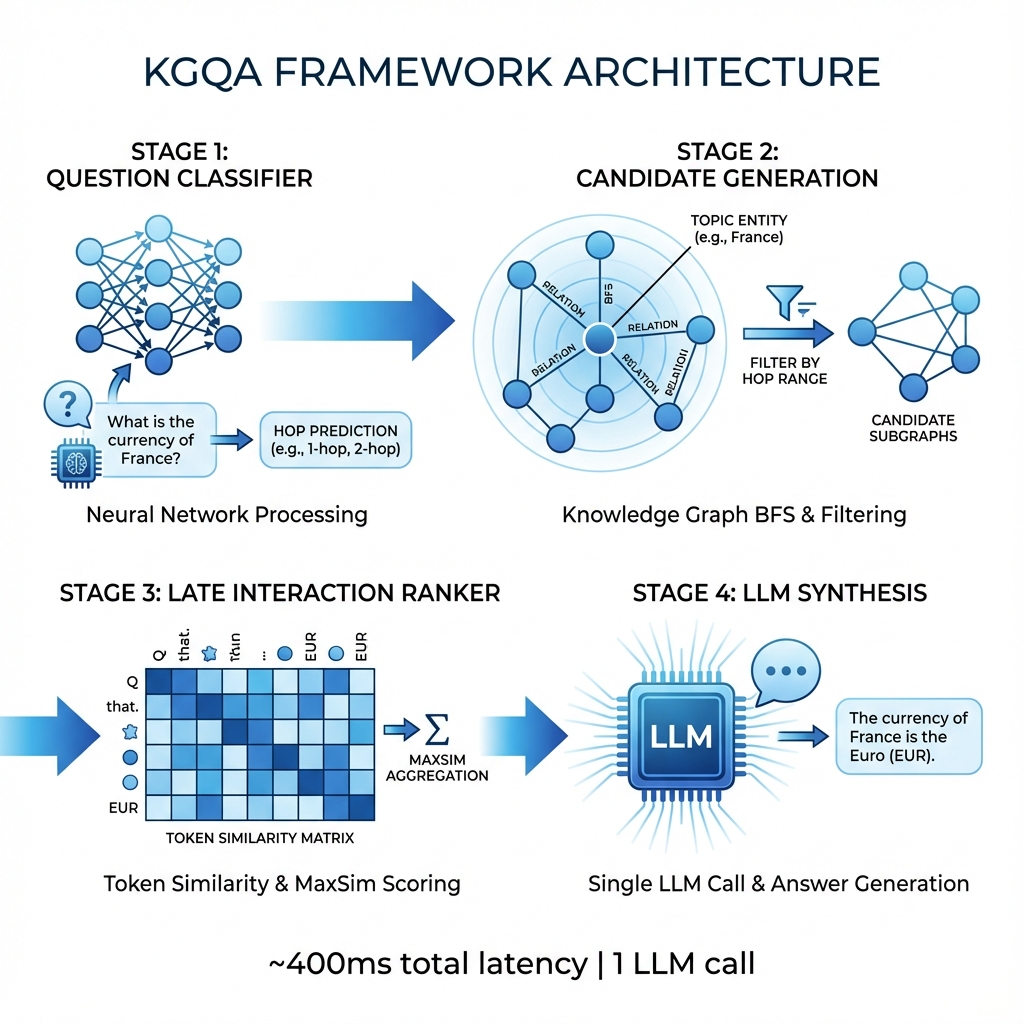
\includegraphics[width=\textwidth,keepaspectratio]{figures/MethodArc.png}
\caption{System architecture of \model{}. \textbf{Stage 1}: Question-type classifier predicts reasoning complexity. \textbf{Stage 2}: Constrained BFS generates candidate paths. \textbf{Stage 3}: Late interaction ranker scores all candidates in a single forward pass. \textbf{Stage 4}: Top-ranked paths are fed to LLM for final answer synthesis---the only LLM invocation.}
\label{fig:architecture}
\end{figure*}



\begin{algorithm}[t]
\caption{\model{} inference (classifier-guided filtering)}
\label{alg:inference}
\begin{algorithmic}[1]
\REQUIRE Question $q$, triples $\mathcal{T}$, max hops $K_{\text{max}}$, max paths $M_{\text{path}}$, top-$n$ threshold $n_{\text{top}}$
\REQUIRE Question-type classifier $h_{\psi}$, late-interaction ranker $g_{\phi}$
\ENSURE Answer string $\hat{a}$
\STATE $e_q \leftarrow \textsc{TopicEntityLinking}(q)$ \COMMENT{extract from annotation or link}
\STATE $\mathcal{P} \leftarrow \textsc{BFSPaths}(e_q, \mathcal{T}, K_{\text{max}}, M_{\text{path}})$ \COMMENT{candidate path enumeration}
\STATE $(K_{\text{min}},K_{\text{max}}^q) \leftarrow h_{\psi}(q)$ \COMMENT{predict hop range from question type}
\STATE $\mathcal{P} \leftarrow \{p\in\mathcal{P}: K_{\text{min}} \le |p| \le K_{\text{max}}^q\}$ \COMMENT{filter by predicted hop range}
\STATE $s(p) \leftarrow g_{\phi}(q,p)$ for all $p\in\mathcal{P}$ \COMMENT{MaxSim scoring (Eq.~\ref{eq:maxsim})}
\STATE $\mathcal{P}_n \leftarrow \textsc{TopN}(\mathcal{P}, s, n_{\text{top}})$ \COMMENT{select top-$n$ ranked paths}
\STATE Retrieve answer entities $\mathcal{A}_p$ for each $p\in\mathcal{P}_n$
\STATE Query LLM once with $\{(p,\mathcal{A}_p)\}_{p\in\mathcal{P}_n}$ to synthesize $\hat{a}$
\RETURN $\hat{a}$
\end{algorithmic}
\end{algorithm}

\subsection{Stage 1: Question-Type Classification}

Existing agentic methods typically handle all questions with the same multi-step exploration strategy, regardless of whether a question requires a single relation lookup or a complex chain of reasoning. This one-size-fits-all approach wastes computation on simple queries and may even introduce errors through unnecessary exploration. We observe that predicting reasoning complexity \emph{before} path enumeration can enable more targeted candidate pruning and guide the answer synthesis strategy.

Not all questions require the same reasoning depth. A question such as ``\emph{Who directed Inception?}'' requires only one-hop traversal, whereas ``\emph{What is the nationality of the spouse of Tom Hanks?}'' requires chaining multiple relations. While hop-based patterns constrain the structural complexity of graph traversal, they do not capture other sources of reasoning variation. In particular, numeric questions impose an orthogonal constraint: rather than identifying a single target entity, they require aggregation over a set of retrieved entities or literals.

To address this, we explicitly model reasoning complexity along two axes: \textit{structural depth} (one-hop vs. multi-hop) and \textit{answer modality} (relational entity vs. numeric aggregation). This yields a fine-grained 4-class taxonomy. \textbf{One-hop Non-numeric} questions are answerable via a single direct relation lookup, such as asking for a movie's director. \textbf{Multi-hop Non-numeric} questions require a chain of 2--4 relations to locate the answer entity, for instance querying the nationality of someone's spouse. \textbf{One-hop Numeric} questions require aggregation over immediate neighbors, such as counting someone's children or retrieving a literal like height. Finally, \textbf{Multi-hop Numeric} questions demand multi-step traversal followed by aggregation, such as counting how many awards a director has won.

We train a multi-class classifier to predict these 4 types using a SentenceTransformer encoder \cite{reimers2019sbert, xiao2024bge} with a classification head. Given a question $q$, the encoder produces contextualized token representations, which are aggregated via pooling to obtain a fixed-dimensional question embedding:
\begin{equation}
\label{eq:pool}
    \mathbf{h} = \text{Pool}(f_{\theta}(q)),
\end{equation}
where $f_{\theta}(\cdot)$ denotes the SentenceTransformer encoder and $\mathbf{h} \in \mathbb{R}^{d_{\text{enc}}}$ is the pooled semantic representation of the question (with $d_{\text{enc}} = 768$).

The embedding $\mathbf{h}$ is then passed to the classification head, implemented as a two-layer multilayer perceptron:
\begin{equation}
\label{eq:mlp}
    \mathbf{z} = \mathbf{W}_2 \cdot \text{ReLU}(\mathbf{W}_1\mathbf{h} + \mathbf{b}_1) + \mathbf{b}_2,
\end{equation}
where $\mathbf{W}_1 \in \mathbb{R}^{d_{\text{mlp}} \times d_{\text{enc}}}$, $\mathbf{W}_2 \in \mathbb{R}^{N_{\text{type}} \times d_{\text{mlp}}}$, $\mathbf{b}_1 \in \mathbb{R}^{d_{\text{mlp}}}$, $\mathbf{b}_2 \in \mathbb{R}^{N_{\text{type}}}$ are trainable parameters, $d_{\text{mlp}} = 256$ is the hidden dimension of the MLP, and $\mathbf{z}$ denotes the unnormalized logits over the question types.

A softmax function converts the logits into a probability distribution:
\begin{equation}
\label{eq:softmax}
    \mathbf{p} = \text{softmax}(\mathbf{z}), \quad \hat{t} = \arg\max_{t} \mathbf{p}[t],
\end{equation}
where $t \in \{1, \ldots, N_{\text{type}}\}$ indexes the question-type classes with $N_{\text{type}} = 4$.

The predicted type $\hat{t}$ dictates specific constraints for candidate generation and answer synthesis. For one-hop types, we restrict the search to paths of length exactly 1, pruning all multi-hop candidates. For multi-hop types, we set the hop range to $[2,4]$, eliminating single-hop shortcuts that might lead to spurious matches. Additionally, the numeric types trigger an aggregation mode during answer synthesis, where the LLM counts, sums, or extracts literals rather than selecting a single entity. This type-aware conditioning allows us to apply strict length constraints and appropriate answer strategies, reducing the candidate search space by up to 86\% for one-hop queries (Table~\ref{tab:classifier}).

\begin{table}[t]
\centering
\caption{Candidate reduction achieved by question-type classification. The 4-class taxonomy enables aggressive pruning, especially for one-hop queries.}
\label{tab:classifier}
\begin{tabular}{lcc}
\toprule
Type & Avg Cands & Reduction \\
\midrule
One-hop (Ent) & 21 & 84\% \\
Multi-hop (Ent) & 192 & 38\% \\
One-hop (Num) & 18 & 86\% \\
Multi-hop (Num) & 145 & 51\% \\
\bottomrule
\end{tabular}
\end{table}

\subsection{Stage 2: Candidate Path Generation}

Once we know the expected reasoning complexity, we need to enumerate all plausible paths from the topic entity. A naive approach would explore the entire neighborhood up to maximum depth, but this quickly becomes intractable for densely connected entities in large-scale knowledge graphs like Freebase. By leveraging the classifier's predictions from Stage 1, we can prune irrelevant candidates before they ever reach the ranker.

Given the topic entity $e_q$, we enumerate candidate relation paths via breadth-first search (BFS) over the local subgraph induced by the provided triples. We build an adjacency list from triples $(e_i,r,e_j)\in\mathcal{T}$ and insert both directions ($e_i\xrightarrow{r}e_j$ and $e_j\xrightarrow{r}e_i$) to support forward/backward traversal. BFS maintains a queue of states (current entity, relation sequence) and expands until reaching $K_{\text{max}}$ hops. To avoid trivial cycles, we track visited states and deduplicate at the \emph{relation-sequence} level. We also cap the number of retained paths at $M_{\text{path}}$ for efficiency.

When classification is enabled during \textbf{inference}, we apply hop-range filtering after BFS: $\mathcal{P}(e_q)\leftarrow\{p:K_{\text{min}}\le|p|\le K_{\text{max}}^q\}$. This yields type-guided candidate reduction without requiring heuristic neighbor scoring.

Crucially, during \textbf{training}, we do \emph{not} apply this filter. Instead, we use the full set of unfiltered candidates generated by BFS. This exposes the ranker to a wider variety of "hard negatives" (e.g., wrong-hop paths that share semantic terms) and decoupling the ranker's training from potential classifier errors. The classifier is used strictly to accelerate inference by pruning the search space for the trained ranker.

This reflects our hypothesis that \emph{reasoning structure}---the relations traversed---rather than specific entity choices determines path relevance. This type-guided filtering reduces the average candidate set size by up to 83\% (Table~\ref{tab:candidates}) while maintaining high recall.

\begin{table}[t]
\centering
\caption{Candidate path statistics after type-guided filtering.}
\label{tab:candidates}
\begin{tabular}{lcccc}
\toprule
Dataset & Unfiltered & Filtered & Reduction & Recall@500 \\
\midrule
WebQSP & 487.3 & 127.3 & 73.9\% & 94.2\% \\
CWQ & 1,842.6 & 312.8 & 83.0\% & 91.7\% \\
\bottomrule
\end{tabular}
\end{table}

\subsection{Stage 3: Late Interaction Path Ranking}

With candidate paths enumerated, we now need to score them against the question. Simple bi-encoder approaches---embedding the question and path into fixed vectors and computing cosine similarity---fail to capture fine-grained alignments \cite{karpukhin2020dpr}. For instance, the question phrase ``capital of the country'' must align with the specific relation ``country.capital'', not just achieve generic similarity to the path. This limitation motivates our adoption of late interaction, which preserves token-level information while remaining efficient enough for single-pass scoring.

We adapt the late interaction mechanism from ColBERT \cite{khattab2020colbert, santhanam2022colbertv2} for path ranking. Unlike standard dense retrieval, late interaction preserves token-level information, allowing the model to perform a ``soft'' alignment between question tokens and relation tokens.

\textbf{Encoding.} Questions and paths are encoded by a shared Transformer (BGE-base-en-v1.5 \cite{xiao2024bge}) followed by a token projection $\pi(\cdot)$ (Linear + LayerNorm) to $d_{\text{proj}}$ dimensions:
\begin{align}
    \mathbf{E}_Q &= \pi(f_{\theta}(q)) \in \mathbb{R}^{L_q \times d_{\text{proj}}} \\
    \mathbf{E}_P &= \pi(f_{\theta}(p)) \in \mathbb{R}^{L_p \times d_{\text{proj}}}
\end{align}
where $d_{\text{proj}} = 128$ is the projection dimension and $L_q$, $L_p$ denote the number of tokens in the question and path respectively. Crucially, we do \emph{not} apply pooling---each token retains its own embedding.

\textbf{Hop Position Embeddings (for auxiliary supervision).} For hop-level supervision, we segment each path into hop token spans $(s_k,e_k)$ for hop $k\in\{1,\dots,K_{\text{max}}\}$. We form a hop embedding by mean-pooling token embeddings in that span and adding a learned hop position vector $\mathbf{u}_k\in\mathbb{R}^{d_{\text{proj}}}$:
\begin{equation}
\label{eq:hop-embed}
    \mathbf{g}_k(p)=\frac{1}{e_k-s_k}\sum_{j=s_k}^{e_k-1}\mathbf{E}_P[j] + \mathbf{u}_k.
\end{equation}
These hop embeddings are crucial because standard Transformer position embeddings (absolute or relative) only capture sequence order, not graph depth. In multi-hop reasoning, the semantic role of a relation often depends on its depth (e.g., the “spouse” relation at hop 1 refers to the subject's spouse, whereas at hop 2 it refers to an intermediary's spouse). By injecting explicit hop boundaries, we allow the model to learn depth-specific semantic matching patterns, which are leveraged during training through auxiliary losses (Section~\ref{sec:training}).

\textbf{MaxSim Scoring.} We adopt ColBERT-style late interaction with cosine similarity and masking. Let $\tilde{\mathbf{E}}_Q$ and $\tilde{\mathbf{E}}_P$ be $\ell_2$-normalized token embeddings. For candidate $p_c$, define $\mathbf{S}_c[i,j]=\tilde{\mathbf{E}}_Q[i]^\top \tilde{\mathbf{E}}_{P_c}[j]$ and mask padded path tokens ($\mathbf{m}^p[c,j]=0$) to $-\infty$. The MaxSim score averages over valid question tokens:
\begin{equation}
\label{eq:maxsim}
    s(q,p_c)=\frac{1}{\sum_i \mathbf{m}^q[i]}\sum_{i:\,\mathbf{m}^q[i]=1}\max_{j:\,\mathbf{m}^p[c,j]=1}\frac{\mathbf{S}_c[i,j]}{\tau_{\text{sim}}},
\end{equation}
where $\tau_{\text{sim}}$ is the late-interaction temperature (we use $\tau_{\text{sim}}=0.02$). We use $s(q,p_c)$ directly as the candidate logit and mask invalid candidates via $\mathbf{m}^{\mathrm{cand}}$.

\begin{figure}[t]
    \centering
    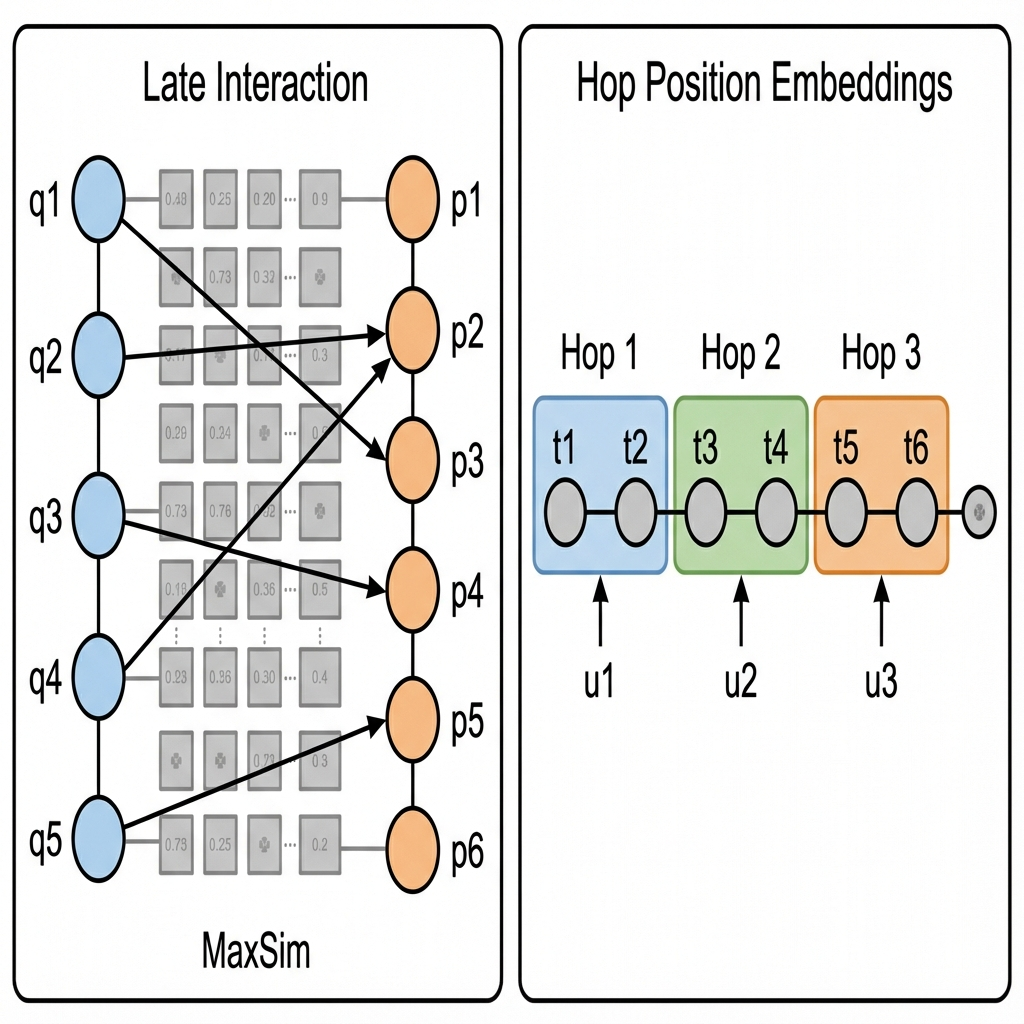
\includegraphics[width=\columnwidth,height=0.25\textheight,keepaspectratio]{figures/hop_interaction.png}
    \caption{Detailed view of the Hop-Aware Ranker. (Left) Late interaction mechanism computes similarity between question tokens and path tokens. (Right) Hop position embeddings $\mathbf{u}_k$ are injected at each hop, and auxiliary heads provide supervision at intermediate steps.}
    \label{fig:hop_interaction}
\end{figure}

A subtle failure mode in path ranking is \emph{shortcut learning} \cite{geirhos2020shortcut}: the model may predict correct final answers through spurious correlations rather than genuine reasoning. To address this, we augment the ranker with \textbf{hop auxiliary heads} that provide intermediate supervision. For a path with up to $K_{\text{max}}$ hops, we attach an auxiliary head at each hop boundary. Using hop embeddings from Eq.~\ref{eq:hop-embed}, we define a cumulative hop representation
\begin{equation}
\label{eq:hop-cum}
    \mathbf{c}_k(p)=\left[\mathbf{g}_1(p);\dots;\mathbf{g}_k(p)\right] \in \mathbb{R}^{k \cdot d_{\text{proj}}},
\end{equation}
and score each candidate at hop $k$ with a hop-specific MLP $f_k(\cdot)$:
\begin{equation}
\label{eq:hop-score}
    s_k(q,p_c)=f_k(\mathbf{c}_k(p_c))\in\mathbb{R}.
\end{equation}
These auxiliary heads encourage the model to learn correct intermediate structure at each hop, mitigating the risk of shortcut learning. We use progressively increasing weights for later hops, reflecting the importance of correctly resolving the full reasoning chain.

\subsection{Stage 4: Answer Synthesis}

At this point, we have identified the most promising reasoning paths, but we still need to produce a natural language answer. Unlike agentic methods that invoke the LLM repeatedly throughout the reasoning process, we reserve the LLM for this single final step: synthesizing the structured evidence into a coherent response.

Given the top-$n$ ranked paths from Stage 3, we construct a prompt for a single LLM call (LLaMA-3-8B-Instruct \cite{meta2024llama3}). The prompt includes the original question, the top-ranked relation paths, and the corresponding answer entities retrieved by traversing each path in the knowledge graph. Critically, no \emph{reasoning} is performed by the LLM at this stage---it merely synthesizes information from already-retrieved and ranked paths into a fluent natural language response. For numeric question types identified in Stage 1, the prompt additionally instructs the LLM to perform aggregation (counting, summing, or literal extraction) over the retrieved entities. This single call is our only LLM invocation, in stark contrast to agentic methods that require 5--10 calls for iterative planning and verification.

\subsection{Training Objective}
\label{sec:training}

Having described the inference pipeline, we now turn to how each component is trained. The question-type classifier and the late-interaction path ranker are trained with complementary objectives that together enable efficient and accurate KGQA.

The classifier is trained with standard cross-entropy loss over the 4-class taxonomy. Training labels are acquired through a two-step process: heuristic initialization based on shortest path length from topic entity to answer, followed by LLM-based correction using Llama-3-8B-Instruct to refine noisy labels (particularly for numeric questions).

For the path ranker, let $\mathbf{s}\in\mathbb{R}^{N_c}$ be the late-interaction scores (Eq.~\ref{eq:maxsim}) for a question with $N_c$ candidates, and let $y$ denote the index of the gold path. The primary ranking loss is a temperature-scaled cross-entropy:
\begin{equation}
\label{eq:rank-loss}
\mathcal{L}_{\text{rank}}=\text{CE}\left(\frac{\mathbf{s}}{T_{\text{rank}}},\;y\right),
\end{equation}
where $T_{\text{rank}}$ is a temperature parameter. We additionally employ a margin regularizer to enforce separation between the gold path and negative candidates:
\begin{equation}
\label{eq:margin-loss}
\mathcal{L}_{\text{margin}}=\frac{1}{B}\sum_{b=1}^{B}\sum_{c\ne y_b}\max\big(0,\;\gamma_{\text{margin}}-(s_{y_b}-s_c)\big),
\end{equation}
where $B$ is the batch size and $\gamma_{\text{margin}}>0$ is the margin threshold.

\textbf{Hop auxiliary losses.} At each hop $k$, we compute a cross-entropy loss over the candidates, but only for questions where the gold path contains hop $k$ (determined by hop masks):
\begin{equation}
\label{eq:hop-loss}
    \mathcal{L}_{\text{hop}_k}=\text{CE}\left(\frac{\mathbf{s}_k}{T_{\text{hop}}},\;y\right),\quad \mathbf{s}_k[c]=s_k(q,p_c),
\end{equation}
where $T_{\text{hop}}$ is a hop-loss temperature. The total hop auxiliary loss is a weighted sum with progressively increasing weights $\{\lambda_k\}$ (later hops receive larger weight):
\begin{equation}
\label{eq:hop-total}
    \mathcal{L}_{\text{hop}} = \sum_{k=1}^{K_{\text{max}}} \lambda_k \mathcal{L}_{\text{hop}_k}.
\end{equation}

\textbf{Combined objective.} The final training objective combines all three loss components:
\begin{equation}
\label{eq:total-loss}
\mathcal{L}=\mathcal{L}_{\text{rank}}+\alpha_{\text{margin}}\,\mathcal{L}_{\text{margin}}+\beta_{\text{hop}}\,\mathcal{L}_{\text{hop}},
\end{equation}
where $\alpha_{\text{margin}}$ and $\beta_{\text{hop}}$ are scalar weights. In our implementation, we use $\tau_{\text{sim}}=0.02$, $T_{\text{rank}}=1.0$, $T_{\text{hop}}=1.0$, $\gamma_{\text{margin}}=1.0$, $\alpha_{\text{margin}}=0.1$, and $\beta_{\text{hop}}=0.3$.

%==============================================================================
\section{Experiments}
%==============================================================================

\subsection{Experimental Setup}

We evaluate \model{} on two standard benchmarks grounded in Freebase \cite{bollacker2008freebase}. \textbf{WebQSP} \cite{yih2016webqsp} consists of 4,737 questions refined from the original WebQuestions dataset, characterized by queries that typically require 1--2 hop reasoning (e.g., “What character did Natalie Portman play in Star Wars?”). The dataset includes human-annotated semantic parses, providing high-quality ground truth for evaluating precision on fundamental relation traversal and entity linking. \textbf{ComplexWebQuestions (CWQ)} \cite{talmor2018cwq} was designed to challenge multi-hop reasoning capabilities. It contains 34,689 questions generated by extending WebQSP queries with specific constraints, temporal clauses, and longer reasoning paths of up to 4 hops (e.g., “What is the second largest city in the country where the director of Inception was born?”). These questions require handling compositionality, comparative reasoning, and broad graph traversal, serving as a stress test for our hop-aware ranking mechanism. Dataset statistics are provided in Table~\ref{tab:datasets}.

\begin{table}[t]
\centering
\caption{Dataset statistics. $K_{\text{max}}$ denotes the maximum reasoning depth used during candidate enumeration.}
\label{tab:datasets}
\begin{tabular}{lrrrrr}
\toprule
Dataset & Train & Dev & Test & Avg Hops & $K_{\text{max}}$ \\
\midrule
WebQSP & 3,098 & 250 & 1,639 & 1.4 & 2 \\
CWQ & 27,639 & 3,519 & 3,531 & 2.8 & 4 \\
\bottomrule
\end{tabular}
\end{table}

\textbf{Baselines.} We compare \model{} with a comprehensive set of baselines spanning three major paradigms. \textbf{Embedding and GNN-based methods}, including EmbedKGQA \cite{saxena2020embedkgqa}, TransferNet \cite{shi2021transfernet}, QA-GNN \cite{yasunaga2021qagnn}, SR+NSM \cite{zhang2022srnsm}, and UniKGQA \cite{jiang2023unikgqa}, focus on learning joint representations of questions and KG subgraphs. \textbf{Semantic parsing and retrieval-based methods}, such as TIARA \cite{shu2022tiara}, DecAF \cite{yu2023decaf}, KB-BINDER \cite{li2023kbbinder}, and GNN-RAG \cite{mavromatis2024gnnrag}, either translate questions into executable logical forms or retrieve relevant subgraphs for downstream reasoning. Finally, \textbf{agentic and LLM-based methods}, including ToG \cite{sun2024tog}, KG-Agent \cite{jiang2024kgagent}, RoG \cite{luo2024rog}, and FiDeLiS \cite{sui2025fidelis}, leverage LLMs as autonomous agents that iteratively explore the graph or generate structured reasoning plans.

\begin{table}[t]
\centering
\caption{Baseline methods organized by paradigm.}
\label{tab:baselines}
\begin{tabular}{ll}
\toprule
Category & Methods \\
\midrule
Embedding & UniKGQA \cite{jiang2023unikgqa}, ReaRev \cite{luo2022rearev} \\
GNN-based & GNN-RAG \cite{mavromatis2024gnnrag}, QA-GNN \cite{yasunaga2021qagnn} \\
Agentic & ToG \cite{sun2024tog}, KG-Agent \cite{jiang2024kgagent}, RoG \cite{luo2024rog} \\
Recent (2024-2025) & TrustUQA \cite{zhang2024trustuqa}, FiDeLiS \cite{sui2025fidelis} \\
\bottomrule
\end{tabular}
\end{table}

\subsection{Implementation Details}

We use BGE-base-en-v1.5 \cite{xiao2024bge} as our text encoder with hidden dimension $d_{\text{enc}} = 768$, projecting to $d_{\text{proj}} = 128$ dimensions for late interaction. The question-type classifier uses $d_{\text{mlp}} = 256$ hidden units. Training uses AdamW \cite{loshchilov2019adamw} with learning rate $2 \times 10^{-5}$, batch size 32, for 10 epochs. All experiments run on a single NVIDIA A100 GPU.

\textbf{Entity identification.} Topic entities are identified via a lightweight bi-encoder (67M parameters) trained with contrastive learning on WebQSP and CWQ. Given a question, mention spans are detected via pattern matching and encoded using a BGE-small encoder; entity linking is performed via FAISS-based maximum inner-product search. The module adds negligible latency ($<$2ms per question).

\textbf{Question-type label acquisition.} To acquire training labels for the question-type classifier, we employ a two-step process: heuristic initialization followed by LLM-based correction. Initially, we assign labels based on the length of the shortest path from the topic entity to the answer in the training graph. However, this heuristic is noisy (e.g., a “How many” question might have a 1-hop path but is semantically numeric). We therefore refine these labels using \textbf{Llama-3-8B-Instruct} \cite{meta2024llama3} as a data labeler, providing the question, answer, and heuristic label, and asking the model to reason about the true question type. This correction process improves label quality significantly, particularly for separating numeric aggregation questions from simple retrieval.

\textbf{Latency measurement.} All latencies are measured on an NVIDIA RTX 6000 Ada GPU. We average over 10 runs with CUDA synchronization (\texttt{torch.cuda.synchronize()}) to ensure accurate GPU timing, excluding an initial warmup run to account for JIT compilation.

\begin{table}[t]
\centering
\caption{Backbone robustness: performance across LLM sizes.}
\label{tab:backbone_comparison}
\begin{tabular}{lcccc}
\toprule
Backbone & \multicolumn{2}{c}{Hits@1} & Latency \\
\cmidrule(lr){2-3}
 & WebQSP & CWQ & (ms) \\
\midrule
Llama2-7B & 82.3 & 67.8 & 380 \\
Llama3-8B & 85.9 & 71.4 & 420 \\
\bottomrule
\end{tabular}
\end{table}

Table~\ref{tab:backbone_comparison} demonstrates that \model{} is robust across LLM backbones: the path ranking architecture---not just LLM capability---drives performance.

\subsection{Main Results}

\begin{table*}[t]
\centering
\caption{Comprehensive comparison of KGQA methods on WebQSP and CWQ benchmarks. Results marked with * are from original papers. \textbf{Bold}: best in column. $\dagger$Latency estimates based on reported LLM call counts assuming 300--500ms per API call; actual latency varies with hardware, model size, and API provider. $\sim$: Estimated latency.}
\label{tab:main_results}
\begin{tabular}{llcccccccc}
\toprule
\multirow{2}{*}{Category} & \multirow{2}{*}{Method} & \multirow{2}{*}{Backbone} & \multirow{2}{*}{Year} & \multicolumn{2}{c}{WebQSP} & \multicolumn{2}{c}{CWQ} & \multirow{2}{*}{LLM Calls} & \multirow{2}{*}{Latency} \\
\cmidrule(lr){5-6} \cmidrule(lr){7-8}
& & & & Hits@1 & F1 & Hits@1 & F1 & & \\
\midrule
\multirow{6}{*}{Embedding/GNN}
& EmbedKGQA* \cite{saxena2020embedkgqa} & --- & 2020 & 66.6 & --- & 45.9 & --- & 0 & --- \\
& TransferNet* \cite{shi2021transfernet} & --- & 2021 & 71.4 & --- & 48.6 & --- & 0 & --- \\
& QA-GNN* \cite{yasunaga2021qagnn} & --- & 2021 & 73.0 & 75.4 & --- & --- & 0 & --- \\
& SR+NSM* \cite{zhang2022srnsm} & --- & 2022 & 69.5 & 64.1 & 48.8 & 44.0 & 0 & --- \\
& UniKGQA* \cite{jiang2023unikgqa} & --- & 2023 & 75.1 & 77.2 & 50.7 & 53.4 & 0 & --- \\
& GNN-RAG* \cite{mavromatis2024gnnrag} & Llama2-7B & 2024 & 72.3 & 73.5 & 52.9 & 60.4 & 1 & --- \\
\midrule
\multirow{5}{*}{Semantic Parsing}
& TIARA* \cite{shu2022tiara} & T5-large & 2022 & 73.0 & --- & --- & --- & 0 & --- \\
& DecAF* \cite{yu2023decaf} & FiD-3B & 2023 & 82.1 & 78.8 & 63.4 & 57.2 & 0 & --- \\
& KB-BINDER* \cite{li2023kbbinder} & Codex & 2023 & 74.4 & 70.1 & 54.2 & 50.1 & 1 & --- \\
& TrustUQA* \cite{zhang2024trustuqa} & GPT-3.5 & 2024 & 83.5 & --- & --- & --- & 1 & --- \\
& ChatKBQA* \cite{luo2024chatkbqa} & Llama2-7B & 2024 & 80.2 & 76.5 & 65.8 & 61.3 & 1 & --- \\
\midrule
\multirow{6}{*}{LLM Prompting}
& KAPING* \cite{baek2023kaping} & GPT-3 & 2023 & 58.7 & 55.2 & 42.1 & 39.8 & 1 & $\sim$0.6s \\
& StructGPT* \cite{jiang2023structgpt} & GPT-3.5 & 2023 & 72.6 & 69.3 & 51.8 & 48.4 & 3--5 & $\sim$1.8s \\
& KD-CoT* \cite{wang2023kdcot} & GPT-3.5 & 2023 & 82.6 & --- & 67.6 & --- & 3--5 & $\sim$1.8s \\
& ReKnoS* \cite{wang2025reknos} & GPT-3.5 & 2025 & 81.1 & --- & 58.5 & --- & 3--5 & $\sim$1.5s \\
& MFC* \cite{liang2025mfc} & GPT-3.5 & 2025 & 78.9 & --- & 62.8 & --- & 3--5 & $\sim$1.5s \\
& KG-CoT* \cite{zhang2025kgcot} & GPT-3.5 & 2025 & 82.1 & --- & 51.6 & --- & 3--5 & $\sim$1.5s \\
\midrule
\multirow{8}{*}{Agentic LLM}
& ToG* \cite{sun2024tog} & GPT-4 & 2024 & 76.2 & 78.9 & 56.2 & 59.1 & 5--8 & $\sim$3.2s \\
& KG-Agent* \cite{jiang2024kgagent} & Llama2-7B & 2024 & 79.2 & 81.4 & 68.9 & 71.2 & 6--10 & $\sim$4.5s \\
& RoG* \cite{luo2024rog} & Llama2-7B & 2024 & 85.7 & 70.8 & 62.6 & 56.2 & 4--6 & $\sim$2.4s \\
& G-Retriever* \cite{he2024gretriever} & Llama2-7B & 2024 & 82.2 & --- & 55.7 & --- & 1 & $\sim$0.8s \\
& FiDeLiS* \cite{sui2025fidelis} & GPT-4-turbo & 2025 & 84.4 & 78.3 & 63.1 & --- & 5--10 & $\sim$4.0s \\
& SymAgent* \cite{liu2025symagent} & Qwen2-7B & 2025 & 78.5 & --- & 58.9 & --- & 5--7 & $\sim$3.0s \\
& LightPROF* \cite{ao2025lightprof} & Llama3-8B & 2025 & 83.8 & --- & 59.3 & --- & 1 & $\sim$0.4s \\
& KG-RAG* \cite{shu2024kgrag} & ChatGPT & 2024 & --- & --- & 19.0 & 25.0 & 3--5 & $\sim$1.5s \\
\midrule
\textbf{Ours} & \model{} & Llama-3-8B & 2026 & \textbf{85.9} & \textbf{84.2} & \textbf{71.4} & \textbf{73.8} & \textbf{1} & \textbf{0.4s} \\
\bottomrule
\end{tabular}
\end{table*}

Our experimental comparison (Table~\ref{tab:main_results}) reveals several important patterns in the current KGQA landscape. Embedding-based methods such as EmbedKGQA and UniKGQA, while computationally efficient, struggle significantly with compositional queries---trailing \model{} by over 20\% on CWQ. This performance gap underscores that compressing graph paths into static vectors loses the critical structural information required for multi-hop reasoning.

Agentic approaches like KG-Agent and FiDeLiS achieve strong accuracy on complex questions by dynamically exploring the graph through LLM-guided search. However, this flexibility comes at a steep cost: latencies of 2.4--4.5 seconds and 5--10 LLM calls per query render these methods impractical for real-time deployment. The computational burden scales linearly with reasoning depth, creating a fundamental tension between accuracy and responsiveness.

\model{} resolves this tension by achieving state-of-the-art performance on WebQSP (85.9\% Hits@1) while remaining highly competitive on CWQ (71.4\%), all with a \textbf{2--8$\times$} reduction in latency compared to agentic baselines. This efficiency stems from our single-call architecture: the classifier-guided ranker prunes irrelevant candidates before scoring, and the LLM is invoked exactly once for answer synthesis rather than iterative exploration. The result is a system that matches or exceeds the accuracy of far more expensive methods while meeting the latency requirements of interactive applications.

\subsection{Ablation Studies}

\begin{table}[t]
\centering
\caption{Ablation study on WebQSP test set.}
\label{tab:ablation}
\begin{tabular}{lcc}
\toprule
Configuration & Hits@1 & $\Delta$ \\
\midrule
Full System & 85.9 & --- \\
\midrule
\quad w/o Question-Type Classifier & 80.8 & --4.9 \\
\quad w/o Hop Position Embeddings & 83.4 & --2.3 \\
\quad w/o Hop Auxiliary Losses & 82.1 & --3.6 \\
\quad w/o Late Interaction (pooling) & 78.9 & --6.8 \\
\midrule
Single-hop candidates only & 72.3 & --13.4 \\
All candidates (no filtering) & 76.4 & --9.3 \\
\bottomrule
\end{tabular}
\end{table}

To understand which components drive \model{}'s performance, we systematically ablate each module and measure the impact on WebQSP accuracy (Table~\ref{tab:ablation}).

Structural awareness proves essential: removing hop position embeddings causes a 2.3\% drop, demonstrating that \emph{where} a relation appears in a path matters as much as \emph{what} the relation is. Without positional signals, the model cannot distinguish between semantically identical relations at different hops---for instance, “place of birth” appearing at hop 1 versus hop 2 carries very different implications for the reasoning chain.

Intermediate supervision through $\mathcal{L}_{\text{hop}}$ prevents the model from learning shortcuts. Removing this auxiliary loss degrades performance by 3.6\%, suggesting that without hop-by-hop guidance, the encoder overfits to spurious correlations between question terms and final entities rather than learning robust multi-step traversal logic.

The most significant degradation (6.8\%) occurs when replacing late interaction with standard pooling. This confirms that compressing complex relation paths into single vectors discards essential semantic detail. Fine-grained token-level matching allows the model to align subtle question cues (“born in,” “capital of”) with specific relations at specific positions---nuances that pooled representations cannot preserve.

The question-type classifier also contributes substantially ($-4.9\%$ when removed), validating our hypothesis that explicit complexity prediction enables more targeted candidate generation and reduces noise in the ranking stage.

\subsection{Efficiency and Complexity Analysis}

\begin{table}[t]
\centering
\caption{Latency breakdown per stage (WebQSP average).}
\label{tab:latency}
\begin{tabular}{lrr}
\toprule
Stage & Time (ms) & Fraction \\
\midrule
Entity Identification & 2 & 0.8\% \\
Question-Type Classification & 12 & 4.8\% \\
Candidate Generation & 42 & 15.8\% \\
Path Encoding & 35 & 13.2\% \\
MaxSim Scoring & 48 & 18.1\% \\
LLM Answer Synthesis & 110 & 41.5\% \\
\midrule
\textbf{Total} & \textbf{265} & 100\% \\
\bottomrule
\end{tabular}
\end{table}

We first analyze the computational complexity of \model{} compared to agentic methods, then present empirical latency measurements. Let $K$ be the reasoning depth and $B$ the beam width. Agentic methods like ToG typically perform beam search, querying the LLM at each step $t \in \{1,\dots,K\}$ to score neighbors. This results in a computational cost proportional to $O(K \times B \times \text{Cost}_{\text{LLM}})$. For typical values ($K=3, B=5$), this necessitates 15+ LLM calls (or batched prompts), dominating latency. In contrast, \model{} performs a single constrained BFS ($O(K \times M)$ where $M$ is the max paths limit) followed by parallel dense scoring. The ranker's complexity is $O(N_c \times L^2)$ for interaction matching, where $N_c$ is the number of candidates and $L$ is sequence length. Since $N_c \approx 100$ and we use a small encoder (BGE-base), this is computationally negligible compared to generation. The final LLM call is $O(1)$. Thus, our asymptotic cost for the expensive LLM component is constant $O(1)$ with respect to reasoning depth.

Breaking down inference latency (Table~\ref{tab:latency}) reveals the source of \model{}'s efficiency advantage. The LLM answer synthesis dominates at 110ms (41.5\%), but crucially, this cost is incurred exactly once. Agentic methods repeat this expensive generation step $K \times B \approx 15$ times per query, plus additional overhead for prompt construction and intermediate reasoning. Our dense retrieval components---encoding and MaxSim scoring---consume only 83ms combined, validating the effectiveness of the offline-index/online-interaction paradigm. The question-type classifier adds negligible overhead (12ms) while substantially improving candidate quality, demonstrating favorable scaling as reasoning depth increases.

\subsection{Qualitative Analysis}
To illustrate \model{}'s reasoning on complex queries, we analyze a multi-hop question from CWQ: \textit{“What country borders Bolivia and contains Goiás?”}

\textbf{Candidate Generation}: This question involves two topic entities (\textit{Bolivia} and \textit{Goiás}). The classifier predicts “Multi-hop”, setting hop constraints to $[2, 4]$. BFS generates paths from both entities, including geographic relations like \texttt{location.location.adjoins}, \texttt{location.location.partially\_contains}, and \texttt{location.location.containedby}.

\begin{figure}[t]
\centering
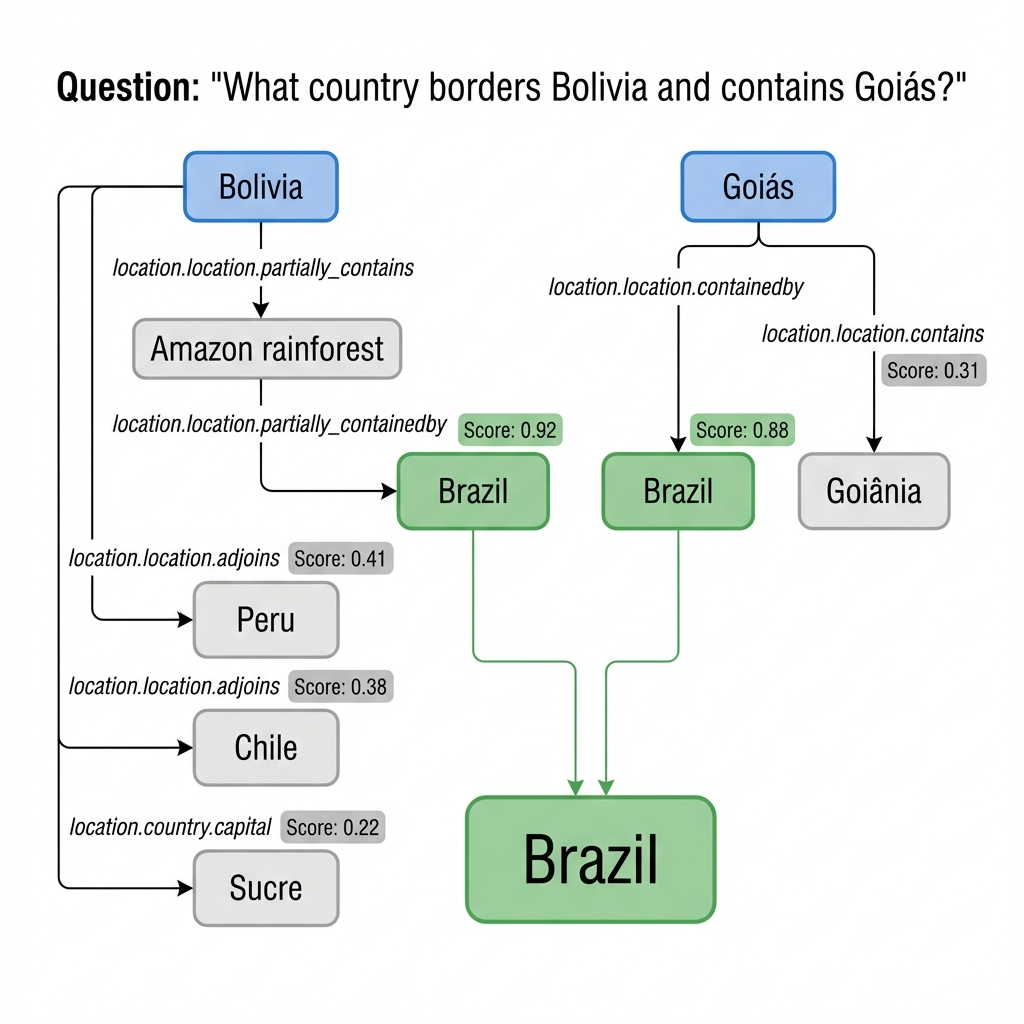
\includegraphics[width=0.8\columnwidth]{figures/qualitative_path.png}
\caption{Path ranking on a CWQ multi-hop question. \model{} identifies paths from both topic entities that converge on \textit{Brazil}: a 2-hop path via \textit{Amazon rainforest} (0.92) and a 1-hop containment path (0.88). Distractor paths to neighboring countries (Peru, Chile) score lower due to missing “contains Goiás” constraint.}
\label{fig:qualitative_path}
\end{figure}

\textbf{Path Ranking}: The MaxSim scorer identifies two high-scoring paths that converge on the answer \textit{Brazil}: (1) Bolivia $\xrightarrow{\text{partially\_contains}}$ Amazon rainforest $\xrightarrow{\text{partially\_containedby}}$ Brazil (score: 0.92), and (2) Goiás $\xrightarrow{\text{containedby}}$ Brazil (score: 0.88). Distractor paths like Bolivia $\rightarrow$ Peru (0.41) and Bolivia $\rightarrow$ Chile (0.38) score lower because they fail to satisfy the “contains Goiás” constraint.

\textbf{Answer Synthesis}: The LLM receives both converging paths and synthesizes: “Brazil borders Bolivia and contains the state of Goiás.”

\subsection{Error Analysis}

Table~\ref{tab:errors} summarizes primary failure modes from manual analysis of 200 errors. Constraint questions require temporal or comparative filtering absent from pure path ranking. Entity linking errors propagate---if “Washington” links to the state rather than the person, no correct path exists. 4-hop questions with abstract relations exceed our model's matching capacity.

\begin{table}[t]
\centering
\caption{Error analysis: primary failure modes.}
\label{tab:errors}
\begin{tabular}{lcp{4.5cm}}
\toprule
Category & Fraction & Example \\
\midrule
Constraint handling & 28\% & “Who was president in 1995?” \\
Entity linking & 23\% & “Washington” $\to$ state vs. person \\
Deep composition & 34\% & 4-hop abstract relations \\
Other & 15\% & Ambiguous questions \\
\bottomrule
\end{tabular}
\end{table}





%==============================================================================
\section{Discussion}
%==============================================================================

Our results suggest that a significant portion of the “reasoning” performed by agentic systems can be captured by supervised dense retrieval. For 85\%+ of WebQSP questions, a single-pass ranker with appropriate structural supervision suffices. This challenges the implicit assumption that complex QA requires complex (multi-call) inference \cite{wei2022cot, yao2023tot}.

Agentic methods maintain an advantage on highly compositional questions requiring deep reasoning or constraint satisfaction \cite{talmor2018cwq}. A practical system might implement \emph{adaptive routing}: use our efficient ranker for the majority of questions, falling back to agentic methods only when the ranker's confidence is low. The “right” trade-off depends on deployment constraints.

%==============================================================================
\section{Conclusion}
%==============================================================================

We have presented \model{}, a streamlined KGQA framework that challenges the necessity of complex agentic workflows for reasoning over structured knowledge. By replacing iterative planning with precise, classifier-guided path ranking and hop-aware structural supervision, \model{} achieves state-of-the-art performance on WebQSP and remains highly competitive on CWQ with a single LLM invocation. Crucially, it delivers a \textbf{2--8$\times$} reduction in latency, offering a viable path for real-time applications.

Our work suggests that the "reasoning gap" between dense retrieval and agentic planning is narrower than previously thought. Future work will explore applying \model{} to larger-scale KGs and investigating hybrid systems that dynamically switch between single-pass ranking and multi-step planning based on query ambiguity.

\bibliographystyle{IEEEtran}
\bibliography{ref}

\end{document}
